\section{Результаты}
\label{sec:Chapter5} \index{Chapter5}
\large



Получена приблизительная сложность работы усовершенствованного алгоритма и в случае случайного графа, модернизация алгоритма дает неплохой результат на небольших размерах. Но эффективность стремительно падает, при увеличении количества вершин графа.

Время работы программы в зависимости от размера графа на среднем по мощности компьютере (затраты оперативной памяти $\thickapprox 2\times 10^9$ байт):
\begin{enumerate}
\item  До 200 вершин - $<$ 1 секунды.
\item  В пределах 300 вершин - около 2 секунд.
\item  400 — 500 вершин - до 20 секунд.
\end{enumerate}




Приблизительная оценка времени работы программы на мощной вычислительной технике:
оперативная память $10^{14}$ байт,
количество операций в секунду $10^{15}$ [5].
\begin{enumerate}
\item 1000 вершин - $<$ 1 секунды  ($10^{12}$  операций).
\item 3000 вершин - $<$ 5 секунд ($5\times 10^{15}$ операций).
\item 10000 вершин - около $2,5$ часов ($10^{19}$ операций).
\item 100000 вершин - около 320000 лет ($10 ^{28}$ операций).
\end{enumerate}
В последнем случае требуется $10^{21}$ байт оперативной памяти.


\begin{figure}[th]
\noindent\centering{
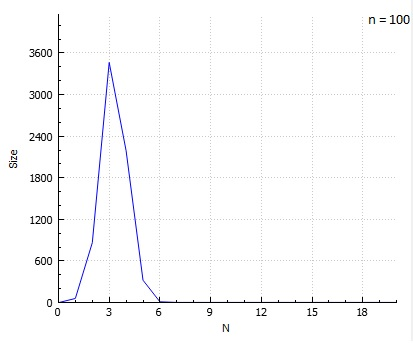
\includegraphics[]{1.jpg}
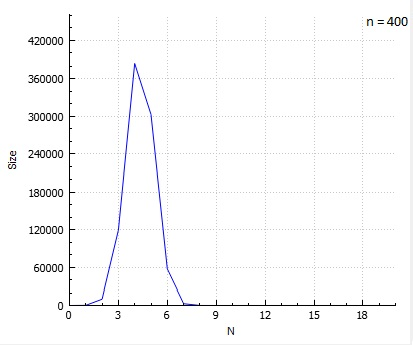
\includegraphics[]{2.jpg}
}
\caption{Построение $\{ |M_m|\} $}
\label{figCurves}
\end{figure}